\documentclass{beamer}

\mode<presentation> {
\usetheme{AnnArbor}
}

\usepackage{graphicx}
\graphicspath{{./figures/}}
\usepackage{caption}
\usepackage{subcaption}
\usepackage{hyperref}
\hypersetup{colorlinks=true}
\usepackage{amsmath}
\usepackage{amsthm}
\usepackage{biblatex}
\addbibresource{bibliography.bib}

\setbeamertemplate{caption}[numbered]

\newtheorem{proposition}{Proposition}
\def\E{\mathbb E}
\def\N{\mathbb N}
\def\P{\mathbb P}
\def\R{\mathbb R}
\def\ind{\perp\!\!\!\perp}
\DeclareMathOperator*{\argmax}{arg\,max}

\newcommand{\CA}{\mathcal{A}}
\newcommand{\CB}{\mathcal{B}}
\newcommand{\CD}{\mathcal{D}}
\newcommand{\CE}{\mathcal{E}}
\newcommand{\CF}{\mathcal{F}}
\newcommand{\CH}{\mathcal{H}}
\newcommand{\CJ}{\mathcal{J}}
\newcommand{\CK}{\mathcal{K}}
\newcommand{\CL}{\mathcal{L}}
\newcommand{\CM}{\mathcal{M}}
\newcommand{\CN}{\mathcal{N}}
\newcommand{\CR}{\mathcal{R}}
\newcommand{\CS}{\mathcal{S}}
\newcommand{\CT}{\mathcal{T}}
\newcommand{\CU}{\mathcal{U}}
\newcommand{\CV}{\mathcal{V}}
\newcommand{\CW}{\mathcal{W}}
\newcommand{\CX}{\mathcal{X}}
\newcommand{\CY}{\mathcal{Y}}

\title[Temporal Point Processes (TPPs)]{Temporal Point Processes (TPPs)}

\author{Aniket Jivani \inst{1} and Victor Verma \inst{2}}
\institute[U-M]{
\inst{1} Department of Mechanical Engineering, University of Michigan \and %
\inst{2} Department of Statistics, University of Michigan
}
\date[12/1/23]{12/1/23}

\begin{document}

\begin{frame}
    \titlepage
\end{frame}

%\begin{frame}{Outline}
%    \tableofcontents
%\end{frame}

\section{Counting Processes}

\begin{frame}{TPP Definition}
    A \textbf{point process} in a space $\mathcal{X}$ is a random countable subset of $\mathcal{X}$. Some special cases:
    \begin{itemize}
        \item $\mathcal{X} = [t_0, \infty)$: a random sequence of times
        \item $\mathcal{X} = \R^3$: a random set of locations
    \end{itemize}
    Let $(\Omega, \mathcal{F}, \P)$ be a probability space. A more formal definition:

    \bigskip

    We will only discuss processes for which $\mathcal{X}$ is of the form $[t_0, \infty)$, i.e., \textbf{temporal point processes} (TPPs).

    \bigskip

    A TPP may have \textbf{marks} or be \textbf{marked}. Marks are extra pieces of information.
    \begin{itemize}
        \item Example: times of earthquakes in California form a TPP; earthquake magnitudes could be marks
    \end{itemize}
\end{frame}

\begin{frame}{Counting Process Definition}
    A given $\omega \in \Omega$ corresponds to some sequence $\{t_n\}_{n = 1}^{\infty}$ in $[t_0, \infty)$. For any $A \subseteq [t_0, \infty)$, set
    \[
    N(A, \omega) = \sum_{n = 1}^{\infty} I(t_n \in A).
    \]
    $N$ is a function from $\mathcal{P}$ to $\N_0$. $N$ is called a \textbf{counting process}.

    \bigskip

    Some notation:
    \begin{itemize}
        \item $N(s, u) := N([s, u))$
        \item $N(t) := N(t_0) + N(t_0, t)$
    \end{itemize}
\end{frame}

\begin{frame}{Notation Continued}
    Drop $\omega$ from counting process notation $\implies$ $N(A)$

    If $A_1, A_2, \cdots$ are disjoint sets in $\mathcal{X}$, 


    $$I_{U_k A_k}(X) = \sum_{k}I_{A_k}(X)$$

    $$I_{U_k A_k}(X) \triangleq N(U_k A_k) = \sum_{i} \sum_{k} I_{A_k}(X_i) = \sum_{k} N_{A_k}$$
\end{frame}

\begin{frame}{Point Process Zoo}
    \begin{figure}
        \centering
        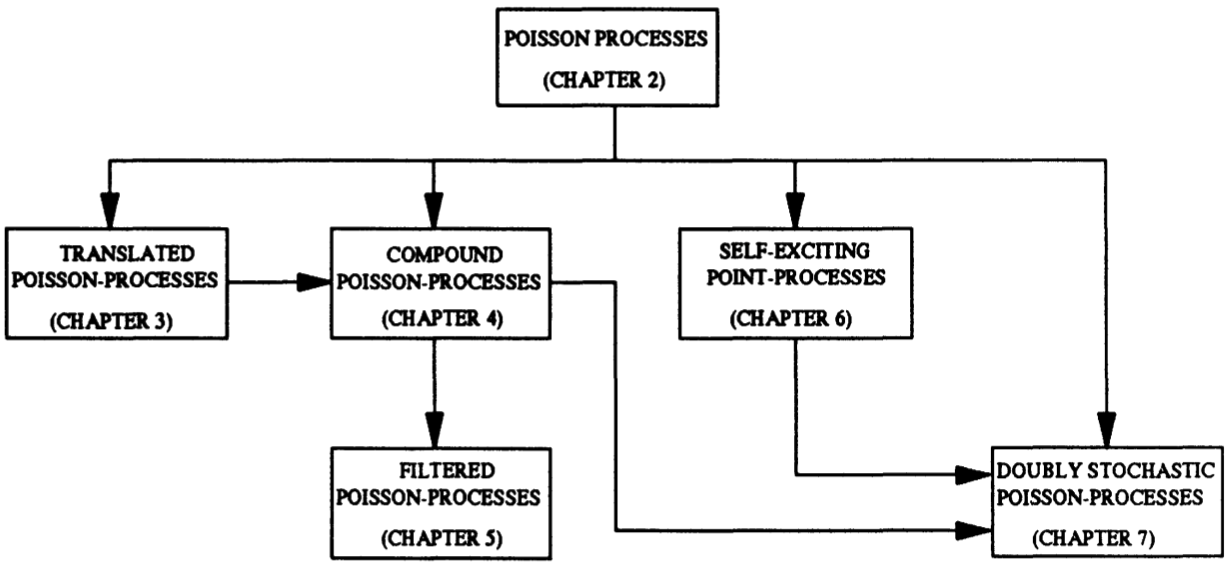
\includegraphics[width=0.8\linewidth]{slides_20231201//figures/pt_process_types.png}
        \caption{From \cite{Snyder_1991}}
        \label{fig:pt_pcs}
    \end{figure}
\end{frame}

% $A = \{t: s \leq t < u \}, \quad t_0 \leq s$
% drop $\omega$ from the counting process notation
% $N(A, \omega)  = N(A) \triangleq N(s, u)$

\begin{frame}{Examples?}
    Random experiment of failure of a light bulb placed in service at $t_0$ i.e. non-denumerable sample space $\Omega = \{\omega: 0 \leq \omega \leq 1\}$

    Other notation: 
    % $\CF$ particular collection of measurable \emph{events} i.e. subsets of $\Omega$
    $\CF$ is the $\sigma$-field or $\sigma$-algebra

    $\mu$ is the probability measure (maps to unit interval $[0, 1]$)

    $x(\omega)$: random variable, $\CR$ is the real line.

    $P_x(X) = \mu(\{\omega: x(\omega) \leq X\})$ - pdf of $x(\omega)$

    Counts: Discrete RV , time intervals - continuous

    \textbf{Stochastic Process:} $\{x(t, \omega): t \in T\}$ family of RVs defined on $(\Omega, \CF, \mu)$, $t$ is index set of process (space, time or both)

    For fixed $t \in T$, $x(t, \omega)$: \textcolor{blue}{$\CR^n$ valued random variable}

    For fixed $\omega \in \Omega$, $x(t, \omega)$: \textcolor{blue}{sample function, relaization, path of process}

    Set of all realizations: \textcolor{blue}{ensemble or sample-function space}
\end{frame}

% This is based on Jakob Rasmussen's lecture notes.
\begin{frame}{Specifying a TPP: Interevent Times}
    An \textbf{interevent time} is a difference between the times of two consecutive events. A TPP can be specified by specifying the conditional distributions of its interevent times.

    \medskip

    Given a TPP $\{\ldots, t_1, t_2, \ldots, t_n\}$, let $\mathcal{H}_t$ represent the history up to time $t$. The history contains information on the times of all events that happen before time $t$. Let $f(t_{n + 1} \mid \mathcal{H}_{t_n})$ be the conditional density of the next event time given the history up to the last event time. Then
    \[
    f(\ldots, t_1, t_2, \ldots)
    = \prod_n f(t_n \mid \ldots, t_{n - 2}, t_{n - 1})
    = \prod_n f(t_n \mid \mathcal{H}_{t_{n - 1}}).
    \]
\end{frame}

% This is based on Jakob Rasmussen's lecture notes.
\begin{frame}{Specifying a TPP: Conditional Intensity Functions}
    It is more intuitive to use \textbf{conditional intensity functions} than interevent times. A TPP is uniquely determined by its conditional intensity function.

    \smallskip
    
    Given $\mathcal{H}_{t_n}$, the corresponding conditional intensity function is defined for $t > t_n$ by
    \[
    \lambda^*(t) = \frac{f(t \mid \mathcal{H}_{t_n})}{1 - F(t \mid \mathcal{H}_{t_n})}.
    \]
    It can be shown that for infinitesimally small $dt$,
    \[
    \lambda^*(t)\,dt = \E[N([t, t + dt]) \mid \mathcal{H}_t],
    \]
    if it is assumed that events do not coincide, i.e., that in an infinitesimally small interval, there is at most one event.
\end{frame}

% This is based on Jakob Rasmussen's lecture notes.
\begin{frame}{Specifying a TPP: Conditional Intensity Functions}
    Some examples:
    \begin{itemize}
        \item \textbf{Inhomogeneous Poisson processes:} letting $\lambda(t)$ be the intensity functions, we have $\lambda^*(t) = \lambda(t)$.
        \item \textbf{Hawkes processes:} These are constructed by defining $\lambda^*$ by
        \[
        \lambda^*(t) = \mu(t) + \alpha\sum_{t > t_i} \gamma(t - t_i; \beta),
        \]
        where $\mu(t) \ge 0$, $\alpha > 0$, and $\gamma(\cdot; \beta)$ is a density on $(0, \infty)$.
        \item \textbf{Self-correcting processes:} Define $\lambda^*$ by
        \[
        \lambda^*(t) = \exp\left(\mu t - \sum_{t > t_i} \alpha\right).
        \]
    \end{itemize}
\end{frame}

% This is based on Jakob Rasmussen's lecture notes.
\begin{frame}{Specifying a TPP: Conditional Intensity Functions}
    A conditional intensity function uniquely determines a TPP under certain conditions:
    \begin{proposition}
        Let $\lambda^*(t)$ be a function such that for any point pattern $(\ldots, t_1, \ldots, t_n)$,
        \begin{enumerate}
            \item $\lambda^*(t) \ge 0$ for all $t > t_n$.
            \item $\lim_{t \to \infty} \int_{t_n}^t \lambda^*(s)\,ds = \infty$.
        \end{enumerate}
        Then $\lambda^*$ uniquely defines a TPP.
    \end{proposition}
\end{frame}

% This is based on Jakob Rasmussen's lecture notes.
\begin{frame}{Specifying a TPP: Conditional Intensity Functions}
    The case of marked TPPs:
\end{frame}

% This is based on Jakob Rasmussen's lecture notes.
\begin{frame}{TPP Likelihoods: No Marks}
    Let $\lambda^*$ be the conditional intensity function of a TPP for which event times $\{t_1, \ldots, t_n\} \subset [0, T)$ have been observed. The \textbf{integrated conditional intensity function} $\Lambda^*$ is defined by
    \[
    \Lambda^*(t) = \int_0^t \lambda^*(s)\,ds.
    \]
    The likelihood function is
    \[
    L(t_1, \ldots, t_n) = \left(\prod_{i = 1}^n \lambda^*(t_i)\right)\exp(-\Lambda^*(T)).
    \]
    {\color{red} Write out the derivation of this on the board?}
\end{frame}

% This is based on Jakob Rasmussen's lecture notes.
\begin{frame}{TPP Likelihoods: Marks}
    If the data is $\{(t_1, \kappa_1), \ldots, (t_n, \kappa_n)\}$, where $\kappa_1, \ldots, \kappa_n$ are marks, then the likelihood function is
    \[
    L(t_1, \ldots, t_n, \kappa_1, \ldots, \kappa_n) = \left(\prod_{i = 1}^n \lambda^*(t_i, \kappa_i)\right)\exp(-\Lambda^*(T)).
    \]
    {\color{red} Write out the derivation of this on the board?}
\end{frame}

\begin{frame}{Sequences and Convergence}
    
\end{frame}

% add more frames, redo sections etc. etc.
\begin{frame}{Poisson Process Organization}
    (Chapters 2, 4, 6)

    \textcolor{blue}{\emph{Temporal Poisson Processes: }} ``Evolve in time without aftereffects i.e. occurrence times and number of points not affected by history of occurrence times and counts.''

    \textcolor{blue}{\emph{Compound / Marked Poisson Processes: }} ``Auxiliary RV called a mark associated with each point occurrence. Can be discrete class labels or real-valued.''

    \textcolor{blue}{\emph{Self-exciting Point Processes: }} ``Can be influenced by full history, but most commonly recent occurrence or total number of past occurrences. Examples - renewal processes and Markov birth processes''
\end{frame}

\section{Temporal Point Processes}
\begin{frame}{Poisson Processes}
    
\end{frame}

\begin{frame}{Hawkes Processes}
    
\end{frame}

\begin{frame}{Simulation Methods}
    
\end{frame}

\section{Applications}
\begin{frame}{Solar Flares}
    
\end{frame}

\begin{frame}{Other Examples}
    
\end{frame}

\section{Neural TPP}
\begin{frame}{STPP}
    \textcolor{red}{we can also avoid STPP and just focus on the neural temporal Hawkes processes to make presentation more focused } - see \cite{jia_neural_2020}

    \emph{Reference for STPP:} RTQ Chen et al. 2020\cite{chen_neural_2020}

    \emph{Key Idea of Neural STPP:} Use Continuous Normalizing Flows (CNFs) to Compute likelihoods for highly complex spatio-temporal distributions

    \emph{Key Idea of Neural SDE:} 

    \textcolor{red}{Provide better motivation behind use of NNs}
\end{frame}

\begin{frame}{Neural ODEs}
    \begin{itemize}
        \item \textbf{Neural ODE:} Continuous update for hidden states of neural networks by passing them through classical ODE solvers. 

        $$\frac{dy}{dt} = f_{\theta}(y(t))$$

        $$y_{t_i} = \textrm{ODESolve}(f, y_{t_0}, t_0, t_i, \theta)$$
    
        \item Loss function updated through integration of adjoint state equation - \emph{constant memory regardless of network depth} i.e. storing intermediate activations is not necessary in forward pass.

        \item Special case of \textcolor{red}{implicit layers} as opposed to the more traditional \textcolor{red}{explicit layers} we normally build in machine learning. The key idea is to \textcolor{blue}{separate the definition and the solution procedure of the layer!} (see \url{http://implicit-layers-tutorial.org}) for examples.
    \end{itemize}
\end{frame}

\begin{frame}{Example Applications}
    \begin{figure}    
    \begin{subfigure}[t]{.45\textwidth}
        \centering
        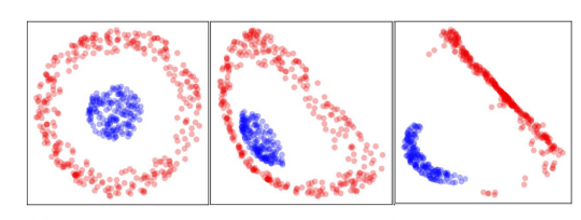
\includegraphics[width=.85\linewidth]{slides_20231201/figures/2d_class_node.png}
        \caption{Building block in e.g. classification \cite{dupont_augmented_2019}}
      \end{subfigure}
      \qquad
      \begin{subfigure}[t]{.45\textwidth}
        \centering
        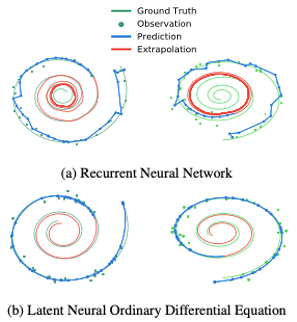
\includegraphics[width=.5\linewidth]{slides_20231201/figures/chen_latent_node.png}
        \caption{Encoder-Decoder latent state \cite{chen2019neural}}
      \end{subfigure}
    
      \medskip
    
      \begin{subfigure}[t]{.45\textwidth}
        \centering
        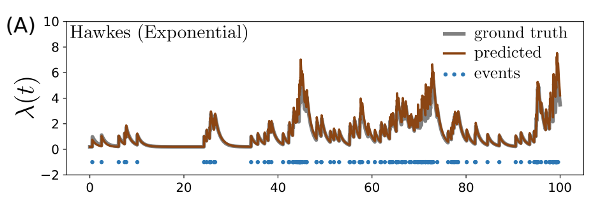
\includegraphics[width=.75\linewidth]{slides_20231201/figures/jia_hawkes.png}
        \caption{Temporal Point Process Model \cite{jia_neural_2020}}
      \end{subfigure}
      \qquad
      \begin{subfigure}[t]{.45\textwidth}
        \centering
        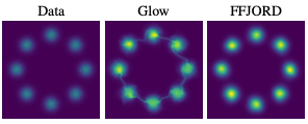
\includegraphics[width=.7\linewidth]{slides_20231201/figures/chen_cnf_2.png}
        \caption{Continuous Normalizing Flows (CNFs) \cite{grathwohl_ffjord:_2018}}
      \end{subfigure}
    \end{figure}
\end{frame}

\begin{frame}{Adjoint formulation}
    \emph{Augmented} loss functional! \footnote{Proof in \cite{chen_neural_2020} is of slightly different flavour, I found this a little more instructive. Paper notation uses $a$ instead of $\lambda$} Introduce \textcolor{red}{Lagrangian multiplier $\lambda$} to form
    
    $$L(u, \lambda, \theta) = \int_{0}^{t_1} g(y, \theta) dt + \int_{0}^{t_1}\lambda(t)^T \left( f - \frac{dy}{dt}\right) dt$$
    
    Choose $\lambda$ to eliminate unwanted terms e.g. those multiplying $\frac{dy}{d\theta}$, simplify and rearrange.

    $$\frac{dL}{d\theta} = \int_{0}^{t_1} \left(\frac{\partial g}{\partial \theta} + \lambda(t)^T \frac{\partial f}{\partial \theta} +   \textcolor{red}{\left( \frac{\partial g}{\partial y} + \lambda^T \frac{\partial f}{\partial y} - \lambda^T \frac{d}{dt}\right)} \frac{dy}{d\theta}\right)dt$$
\end{frame}

\begin{frame}{Adjoint formulation}
    Integration by parts:
    $$\begin{aligned}\int_{0}^{t_1} \lambda^T \frac{d}{dt}\frac{dy}{d\theta} &= \lambda^T(0) \frac{dy_0}{d\theta} - \lambda^T (t_1)\frac{dy(t_1)}{d\theta} + \int_{0}^{t_1}\left( -\frac{d\lambda^T}{dt}\right)\frac{dy}{d\theta}dt\end{aligned}$$

    Plug back into original:

    $$\frac{dL}{d\theta} = \int_{0}^{t_1} \left(\frac{\partial g}{\partial \theta} + \lambda(t)^T \frac{\partial f}{\partial \theta} + \textcolor{red}{\left( \frac{\partial g}{\partial y} + \lambda^T \frac{\partial f}{\partial y} + \left(\frac{d\lambda^T}{dt}\right)\right)} \frac{dy}{d\theta}\right)dt$$
    
    $$+ \lambda^T(0) \frac{dy_0}{d\theta} \textcolor{red}{- \lambda^T (t_1)\frac{dy(t_1)}{d\theta}}$$
\end{frame}

\begin{frame}{Adjoint formulation}
Cancel terms: Solve a terminal-value problem for $\lambda^T$ with terminal condition $\lambda^T(t_1)=0$ and:

$$\left( \frac{\partial g}{\partial y} + \lambda^T \frac{\partial f}{\partial y} + \left(\frac{d\lambda^T}{dt}\right)\right) = 0$$ i.e.

$$\frac{d\lambda}{dt} = -\left(\frac{\partial g}{\partial y}\right)^T - \frac{\partial f}{\partial y}^T \lambda$$

Remaining expression (plug computed $\lambda$):

$$\frac{dL}{d\theta} = \int_{0}^{t_1} \left(\frac{\partial g}{\partial \theta} + \lambda^T \frac{\partial f}{\partial \theta}\right)dt + \lambda^T(0) \frac{dy_0}{d\theta}$$ 
\end{frame}

\begin{frame}{Adjoint formulation}
Key steps:

\begin{enumerate}
    \item Solve $y(t_1) = \textrm{ODESolve}(f, 0, t_1, \theta)$
    
    \item Solve $\frac{d\lambda}{dt} = -\left(\frac{\partial g}{\partial y}\right)^T - \frac{\partial f}{\partial y}^T \lambda$ with $\lambda(t_1)=0$ and $\frac{\partial g}{\partial y(t_1)}$ \textcolor{blue}{Get $y$ while solving backwards: checkpointing, or use time reversible ODE $\frac{dy}{dt} = -f(y, -t)$ to avoid storing intermediate $y(t)$ 
    % \footnote{Not all integrators are time-reversible!}
    \footnote{For examples of other approaches, see slide 35 of \href{https://elliit.se/wp-content/uploads/2022/06/ELLIIT_FP2022_Lund_Chris_Rackauckas.pdf}{Data-Efficient Model Discovery with SciML}}
    }
    
    \item Solve $$\frac{dL}{d\theta} = \int_{0}^{t_1} \left(\frac{\partial g}{\partial \theta} + \lambda^T \frac{\partial f}{\partial \theta}\right)dt + \lambda^T(0) \frac{dy_0}{d\theta}$$ \textcolor{blue}{To calculate integral, store intermediate $\lambda$ or can solve $\mu' = \frac{\partial g}{\partial \theta} + \lambda^T \frac{\partial f}{\partial \theta}$ with $\mu(t_1)=0$}
\end{enumerate}

\end{frame}

\begin{frame}{Forward and Backward Pass}
    \textbf{Implementation pseudocode:} 
    
    \texttt{from torchdiffeq import odeint\textunderscore adjoint as adjoint}

    \texttt{model=MyNeuralNet()}

    \texttt{y=odeint(model, y0, t, solver=`dopri5', atol=1e-5, rtol=1e-4)}

    \texttt{loss= \ldots}

    \texttt{loss.backward()}
\end{frame}


\begin{frame}{Some context}
    Reference: \cite{Nan2016}

    \begin{itemize}
        \item IID and time-series data: Time and space \textcolor{red}{index the data}, typically not RVs

        \item \emph{Event Data}: Online purchases, ridesharing, healthcare records, extreme weather events (e.g. earthquakes) - \textcolor{red}{event timings and / or spatial position and markers become important}

        \item Challenges of forecasting, decision making under uncertainty

        \item Markov models - cannot capture heterogeneity of time intervals, or unable to incorporate long dependencies on history
    \end{itemize}
\end{frame}

\begin{frame}{Notation (Marked Process)}
    \begin{enumerate}
        \item $\mathcal{H} = \{(\tau_j, \mathbf{k}_j)\}$: $\mathbf{k}_j \in \{0, 1\}^m$ for $m$ discrete events \textbf{OR} $\mathbf{k}_j \in \mathbb{R}^m$
        \item $N(t) = \Sigma_{\tau_j \in \mathcal{H}} H(t - \tau_j)$ where $H(t) = \begin{cases}
               0 \quad t \leq 0\\
               1 \quad \text{ otherwise}\\
            \end{cases}$: counting process or counting function

        \item \textbf{Conditional intensity function:} $\lambda_t \cdot dt = p(t_i \in [t, t + dt] | \mathcal{H}_t)$

        \item Latent state of system $\mathbf{z}(t) \in \mathbb{R}^n$ - evolves with a deterministic trajectory until interrupted by a stochastic event.

        $$d\mathbf{z}(t) = f(\mathbf{z}(t), t; \theta) \cdot dt + w (\mathbf{z}(t), \mathbf{k}(t), t; \theta) \cdot dN(t)$$
    \end{enumerate}
\end{frame}

\begin{frame}{Parametrizations}
    $$\lambda^{\ast}(t) = \lim_{dt \rightarrow 0} \frac{P(t < T < t + dt)}{P (T > t)dt}$$

    $$\implies \lambda^{\ast}(t) = \frac{f^{\ast}(t)dt}{1 - F^{\ast}(t)}$$

    where $S^{\ast}(t) = 1 - F^{\ast}(t)$ is the survival probability or the probability that no new event has happened upto $t$ since last event time, say $t_n$ and $f(t)$ is pdf of $T$, where $T$ is an arbitrary time. \textcolor{red}{$\ast$ denotes dependence on time history}

    Finally, from definition of $S(t)$ and chain rule for derivatives, 

    $$\lambda^{\ast}(t) = \frac{f^{\ast}(t)dt}{S^{\ast}(t)} = - \frac{d \log S^{\ast}(t)}{dt}$$

    and \textcolor{red}{by definition?} $S^{\ast}(t) = \exp \left( - \int_{t_n}^{t} \lambda^{\ast}(\tau) d\tau \right)$, $\int_{t_n}^{t} \lambda^{\ast}(\tau) d\tau = \Lambda(t)$ or the \textcolor{red}{Cumulative Hazard Function!}
\end{frame}

\begin{frame}{Modeling the log-likelihood}
If $\mathcal{H}=\{(t_i,\boldsymbol{x}_i)\}_{i=1}^n$ is the sequence of event times and their associated locations, 
then the log-likelihood of $\mathcal{H}$ in a time interval of $[0, T]$ is given by \textcolor{red}{show sketch of derivation}

\begin{equation*}
    \log p\left(\mathcal{H}\right)=\sum_{i\operatorname{-}1}^n\log\lambda^*(t_i,\boldsymbol{x}_i)-\int_0^T\int_{\mathbb{R}^d}\lambda^*(\tau,\boldsymbol{x})\mathrm{~}d\boldsymbol{x}d\tau 
\end{equation*}
\end{frame}

\begin{frame}{Limitations of point process approaches}
    Reference:  \cite{Nan2016}
    \begin{enumerate}
        \item \textbf{Model misspecification} - assuming linearly additive influences from past events, stationarity etc. \textcolor{red}{examples where these assumptions break down?}

        \item \textbf{Marker generation} - require simplifications such as assuming the independence of history for markers, or model a separate temporal process for each marker - this results in a very sparse problem where there are few individual events per unique marker.
    \end{enumerate}
\end{frame}

\begin{frame}{First attempt: Recurrent Nets}
    Reference: \cite{Nan2016}
    RNNs - hidden units incorporate new data as well as state information at each timestep, can model arbitrary length sequences.

    \begin{figure}
        \centering
        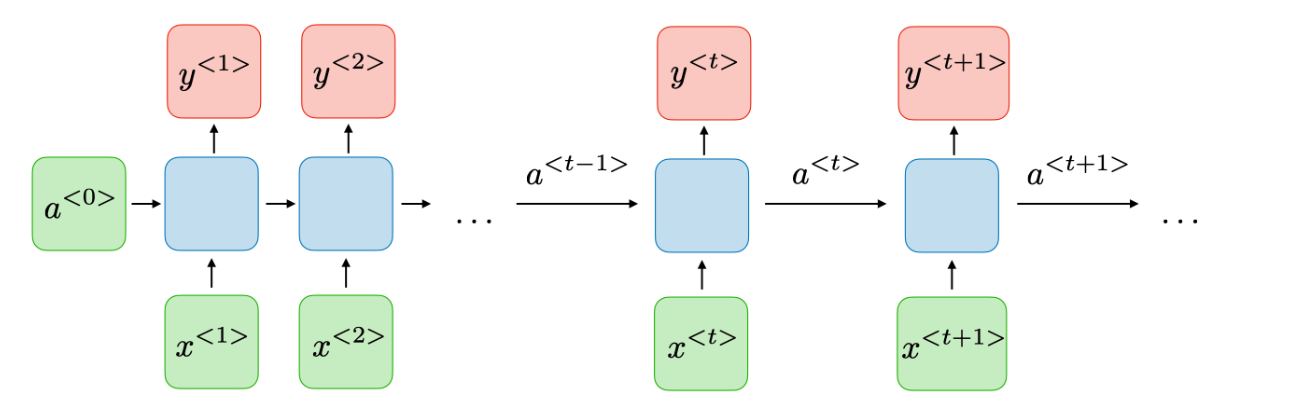
\includegraphics[width=0.7\linewidth]{slides_20231201//figures/rnn_arch_sfcs.png}
        \caption{Generic RNN Architecture \href{https://stanford.edu/~shervine/teaching/cs-230/cheatsheet-recurrent-neural-networks}{Stanford CS-230}}
        \label{fig:rnn_arch}
    \end{figure}

    $a^{<t>}=g_1(W_{aa}a^{<t-1>}+W_{ax}x^{<t>}+b_a)\, \quad y^{<t>}=g_2(W_{ya}a^{<t>}+b_y)$

    BPTT (Backpropagation through time) \textcolor{red}{See \url{https://mmuratarat.github.io/2019-02-07/bptt-of-rnn}}
    
    LSTMs: special gates or units to control problem of vanishing gradients. \cite{hochreiter_2009}
\end{frame}

\begin{frame}{Proposed Architecture}
    \begin{columns}
        \begin{column}{0.4\textwidth}
            Reference: \cite{Nan2016}
            \begin{figure}
                \centering
                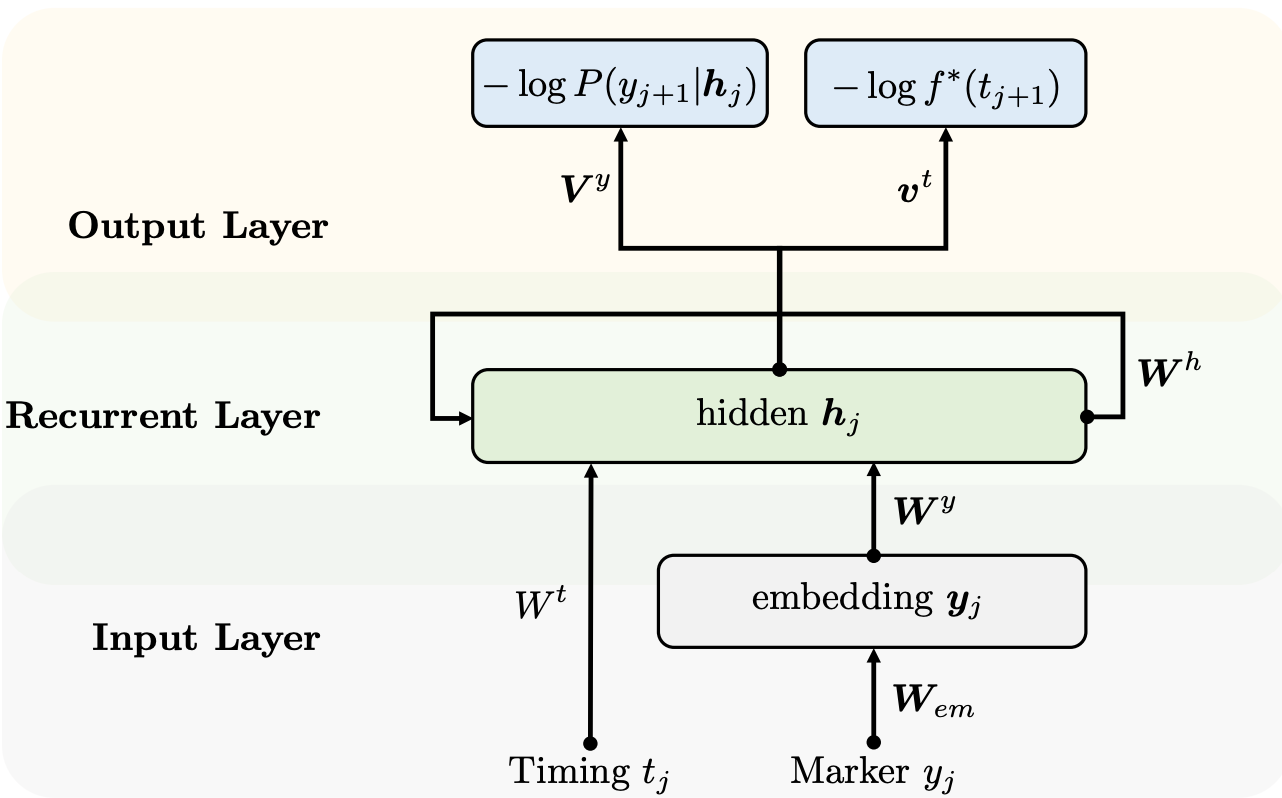
\includegraphics[width=0.97\linewidth]{slides_20231201//figures/recurrent_tpp_nan.png}
                % \caption{Enter Caption}
                \label{fig:rmtpp}
        \end{figure}
    \end{column}

    \begin{column}{0.58\textwidth}
            % \textbf{Update Procedure} for $\mathcal{S} = \left((t_j, y_j)_{j=1}^{n} \right)$
            
            \textcolor{blue}{Hidden layer:} 
            
            $\boldsymbol{h}_j=\max\left\{\boldsymbol{W}^y\boldsymbol{y}_j+\boldsymbol{W}^t\boldsymbol{t}_j+\boldsymbol{W}^h\boldsymbol{h}_{j-1}+\boldsymbol{b}_h,0\right\}$

            \textcolor{blue}{Marker gen: (multinomial)}
            $P(y_{j+1}=k|\boldsymbol{h}_j)=\frac{\exp\left(\boldsymbol{V}_{k,\cdot}^y\boldsymbol{h}_j+b_k^y\right)}{\sum_{k=1}^K\exp\left(\boldsymbol{V}_{k,\cdot}^y\boldsymbol{h}_j+b_k^y\right)}$

            $\lambda^*(t)=\exp(\underbrace{\boldsymbol{v^t}^\top\cdot\boldsymbol{h_j}}_{\text{past influence}}+\underbrace{w^t(t-t_j)}_{\text{current influence}}+\underbrace{b^t}_{\text{base intensity}})$

            \textcolor{blue}{Likelihood}
            $f^*(t)=\lambda^*(t)\exp\left(-\int_{t_j}^t\lambda^*(\tau)d\tau\right)$

            \textcolor{blue}{Given sequences $\mathcal{C}=\{\mathcal{S}^i\}$}, maximize:

            $\ell(\{\mathcal{S}^i\})=\sum_i\sum_j\left(\log P(y_{j+1}^i|\boldsymbol{h}_j)+\log f(t_{j+1}^i|\boldsymbol{h}_j)\right)$
            
    \end{column}
    \end{columns}
\end{frame}

\begin{frame}{Continuous Depth Extension}
    \begin{itemize}
        \item System of interest evolves continuously with time, but may also be interrupted by stochastic events!

        \item Model continuous flow and influence of the jump i.e. event conditional intensity by separate networks, \textcolor{red}{but retain adjoint-based training advantage.}

        \item Learnt model can approximate intensity function for a number of classical point processes such as Hawkes and STPPs. \cite{jia_neural_2020,chen_neural_2020}
    \end{itemize}
\end{frame}

% \begin{frame}{Example}
    
% \end{frame}

% \begin{frame}{Continuous Normalizing Flows}
%     Change of variables

%     Computational difficulty (show highly constrained architectures)

%     Speed up through CNF
% \end{frame}

% \begin{frame}{Example}
%     Gaussian to multi-modal distribution
% \end{frame}






\begin{frame}{Continuous Depth Extension: Approximations}
    \begin{figure}
        \centering
        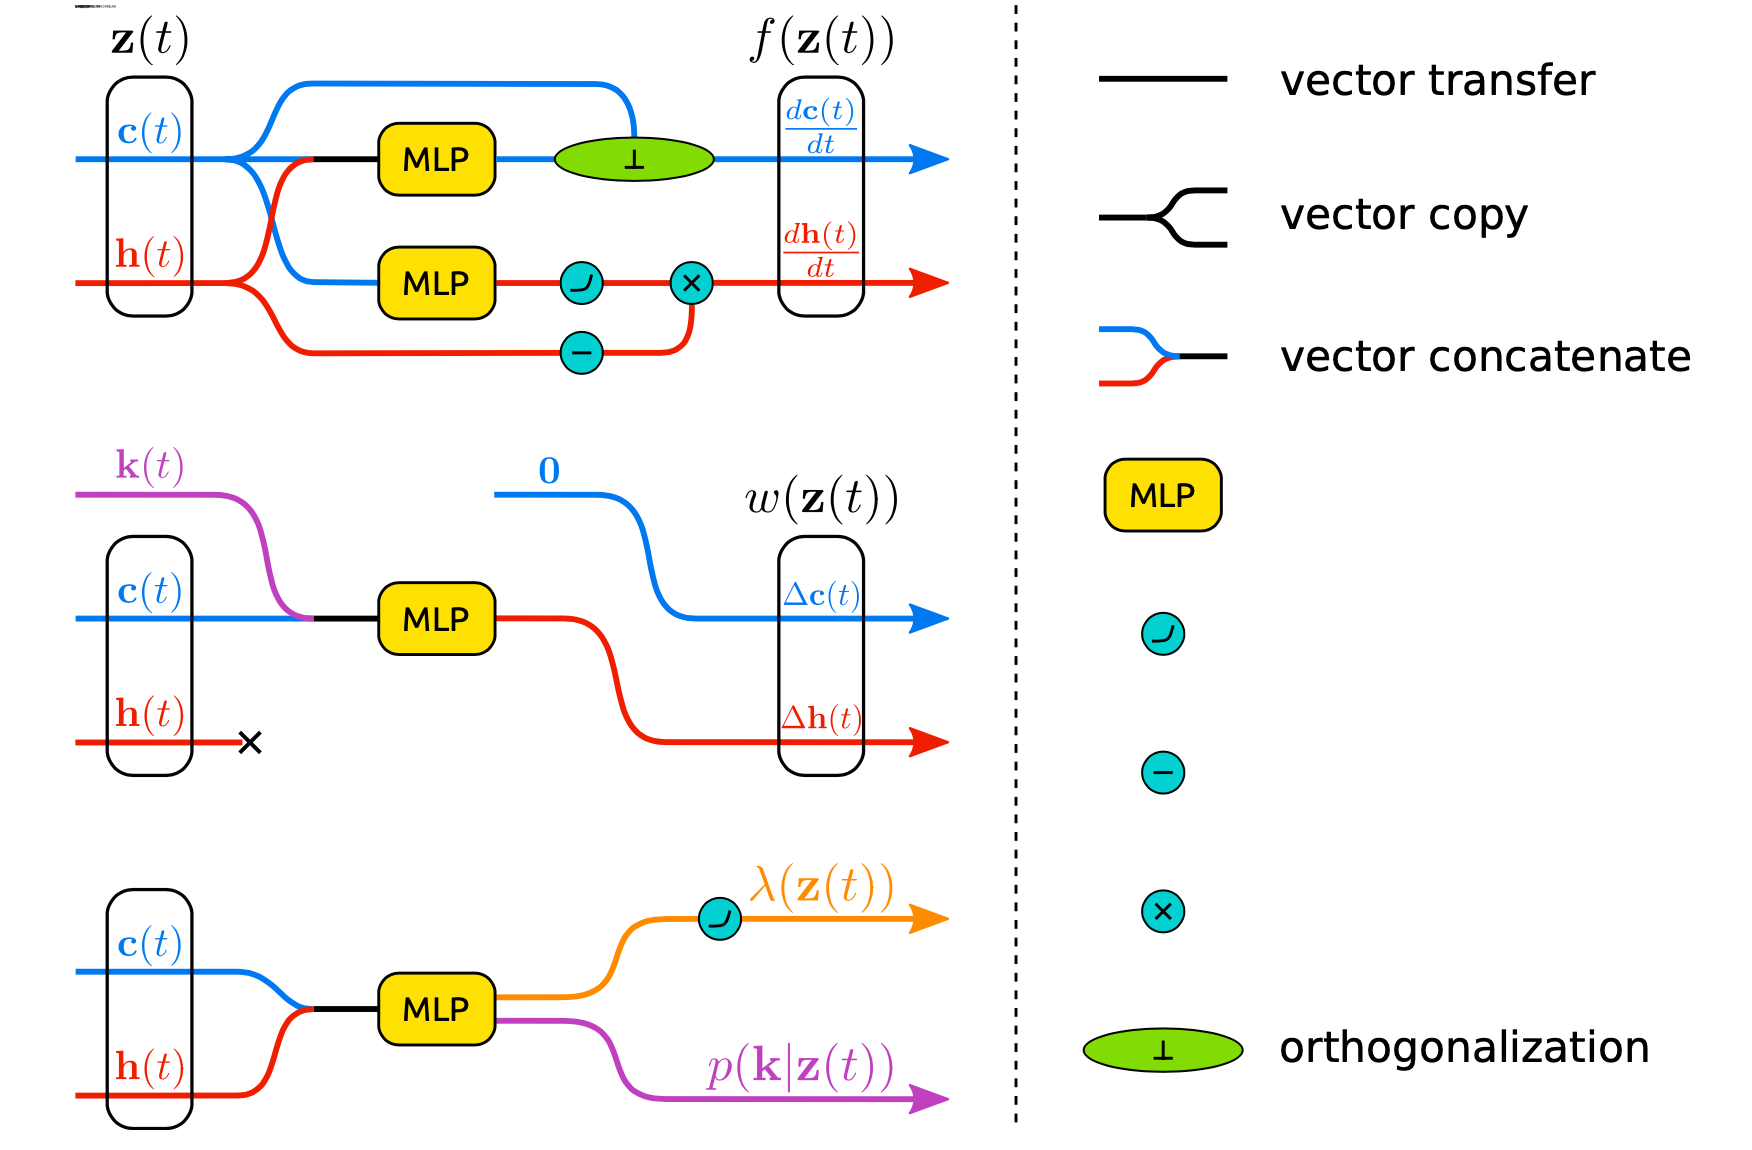
\includegraphics[width=0.75\linewidth]{slides_20231201//figures/NJSDE_Architectures.png}
        \caption{From \cite{jia_neural_2020}}
        \label{fig:njsde_arch}
    \end{figure}
\end{frame}

\begin{frame}{Approximations}
\begin{itemize}
    \item $f$ and $w$ control the flow and the jump respectively

    \item Let $\theta$ be the model parameters
\end{itemize}
    
\end{frame}

\begin{frame}{Algorithm}
    \begin{enumerate}
        \item Loss function

        \item Adjoint sensitivity analysis with discontinuities
    \end{enumerate}
\end{frame}

% \begin{frame}{Proposed framework 2}

% \end{frame}

% \begin{frame}{Proposed framework 3}


% \end{frame}

% \begin{frame}{STPP Definition}



% The conditional intensity function of a spatio-temporal point process i.e. the instantaneous probability of the $i$th event occuring at time $t$ and position $\boldsymbol{x}$ \emph{given $i-1$ events} is specified by:

% \begin{equation*}
% \lambda^{\ast}(t, \boldsymbol{x}) = \lambda(t,\boldsymbol{x}\mid\mathcal{H}_t)\triangleq\lim_{\Delta t\downarrow0,\Delta\boldsymbol{x}\downarrow0}\frac{\mathbb{P}\left(t_i\in[t,t+\Delta t],\boldsymbol{x}_i\in B(\boldsymbol{x},\Delta\boldsymbol{x})\mid\mathcal{H}_t\right)}{|B(\boldsymbol{x},\Delta\boldsymbol{x})|\Delta t}
% \end{equation*}

% \end{frame}

\begin{frame}{Modeling the log-likelihood}
If $\mathcal{H}=\{(t_i,\boldsymbol{x}_i)\}_{i=1}^n$ is the sequence of event times and their associated locations, 
then the log-likelihood of $\mathcal{H}$ in a time interval of $[0, T]$ is given by \textcolor{red}{(show sketch of derivation)}

\begin{equation*}
    \log p\left(\mathcal{H}\right)=\sum_{i\operatorname{-}1}^n\log\lambda^*(t_i,\boldsymbol{x}_i)-\int_0^T\int_{\mathbb{R}^d}\lambda^*(\tau,\boldsymbol{x})\mathrm{~}d\boldsymbol{x}d\tau 
\end{equation*}
\end{frame}

% \begin{frame}{Typical Solution Techniques}
    
% \end{frame}

% \begin{frame}{Approximations}
% \begin{enumerate}
%     \item Decompose conditional intensity function
%     $$\lambda^*(t,\boldsymbol{x})=\lambda^*(t)\not p^*(\boldsymbol{x}\mid t)$$
%     \item Simplify log-likelihood:
%     $$\log p(\mathcal{H})=\underbrace{\sum_{i=1}^n\log\lambda^*(t_i)-\int_0^T\lambda^*(\tau)}_{\text{temporal log-likelihood}}+\underbrace{\sum_{i=1}^n\log p^*(\boldsymbol{x}_{t_i}^{(i)}|t_i)}_{\text{spatial log-likelihood}}$$
%     \item Time varying CNF or jump CNF
% \end{enumerate}
    
% \end{frame}

\begin{frame}{Results}
    Compare ground truth and predicted conditional intensities:

    $$\frac1{t_1-t_0}\int_{t_0}^{t_1}dt\left|\frac{\lambda_{\mathrm{model}}^*(t)-\lambda_{\mathrm{GT}}^*(t)}{\lambda_{\mathrm{GT}}^*(t)}\right|\times100\%$$
\end{frame}

\begin{frame}{Real-valued Event Feature Prediction}
    \begin{itemize}
        \item Hawkes process with exponential kernel

        \item Time and location of earthquakes above a threshold in 10 year period (Dataset: \url{www.kaggle.com/danielpe/earthquakes})
    \end{itemize}
    
\end{frame}

\begin{frame}[allowframebreaks]
    \frametitle{References}
    \nocite{*}
    \printbibliography
\end{frame}

\section{Backup}
\begin{frame}{More details on the Adjoint Method}

    Let $G: \R^n \rightarrow \R$ be represented as a composition:
    $$G(x) = g^N \circ g^{N-1} \circ \cdots \circ g^1(x)$$

    and let $h_i$ represent hidden layers.

    If we consider truncated compositions of the form $G^{i:n}(h_i) = g^N \circ g^{N-1} \circ \cdots \circ g^{i + 1}(h_i)$, the gradient for $G$ w.r.t. $x$ can be found using multipliers of the form:

    \begin{equation}
    \label{nablastep}
    \nabla_{\! h_{i}} G^{i:N}=\nabla_{\! h_{i+1}}G^{i+1:N}\cdot \frac{\partial g^{i+1}}{\partial h_{i}}.
    \end{equation}
\end{frame}

\begin{frame}{Adjoint Method - P2}
    
\end{frame}

\begin{frame}{Adjoint Method - P3}
    
\end{frame}

\begin{frame}{Adjoint Method - P4}
    
\end{frame}

\begin{frame}{BPTT - Backpropagation through time}
    
\end{frame}

\end{document}